\documentclass[tikz,border=6pt]{standalone}
\usepackage{amsmath}
\usepackage{xcolor}
\usetikzlibrary{arrows.meta}

\definecolor{axisgray}{HTML}{333333}
\definecolor{lineblue}{HTML}{4A90D9}
\definecolor{linered}{HTML}{E74C3C}

\begin{document}
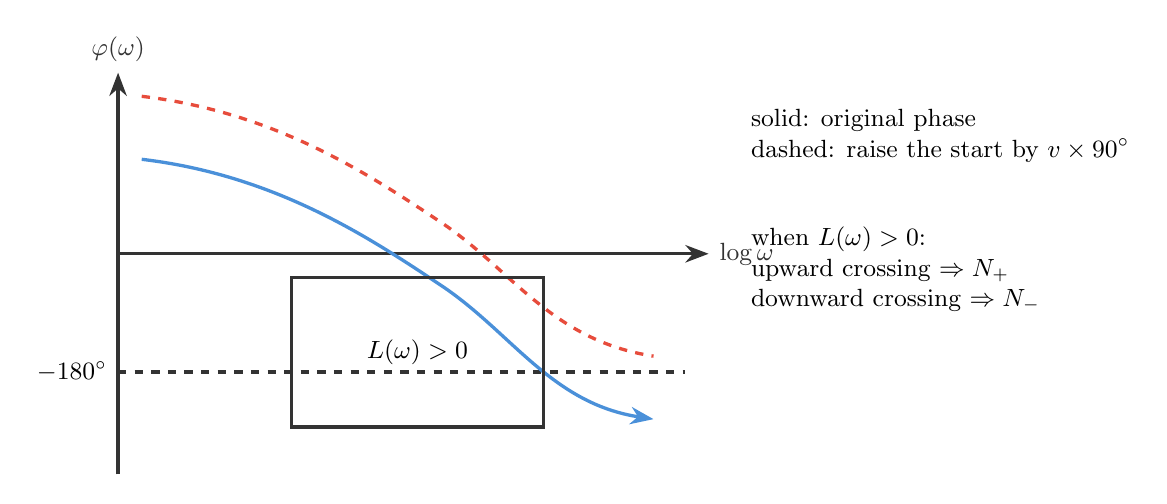
\begin{tikzpicture}[>=Stealth, line width=1.2pt, font=\small]
  \draw[axisgray, ->] (0,0) -- (7.5,0) node[right] {$\log \omega$};
  \draw[axisgray, ->] (0,-2.8) -- (0,2.3) node[above] {$\varphi(\omega)$};
  \draw[axisgray, dashed] (0,-1.5) -- (7.2,-1.5);
  \node[left] at (0,-1.5) {$-180^\circ$};
  \draw[lineblue, ->] (0.3,1.2) .. controls (2.0,1.0) and (3.2,0.2) .. (4.1,-0.4)
    .. controls (5.0,-1.0) and (5.5,-1.9) .. (6.8,-2.1);
  \draw[linered, dashed] (0.3,2.0) .. controls (2.0,1.8) and (3.2,1.0) .. (4.1,0.4)
    .. controls (5.0,-0.2) and (5.5,-1.1) .. (6.8,-1.3);
  \draw[axisgray] (2.2,-2.2) rectangle (5.4,-0.3);
  \node at (3.8,-1.25) {$L(\omega)>0$};
  \node[align=left, anchor=west] at (7.9,1.5) {
    solid: original phase\\
    dashed: raise the start by $v\times 90^\circ$
  };
  \node[align=left, anchor=west] at (7.9,-0.2) {
    when $L(\omega)>0$:\\
    upward crossing $\Rightarrow N_+$\\
    downward crossing $\Rightarrow N_-$
  };
\end{tikzpicture}
\end{document}
